% =============================================================================
% APGCC baseline 复现  (三数据集: BCData / MoNuSeg / CoNIC)
% 依赖宏包: graphicx, booktabs, amsmath, float, multirow, (建议) caption
% 若单独编译, 主文档需: \usepackage{graphicx,booktabs,amsmath,float,multirow}
%   并设置 \graphicspath{{figures/}}
% 本节只涉及 baseline 复现, 不含任何优化 / 模块集成内容.
% =============================================================================

\subsubsection{APGCC复现}

\begin{enumerate}
    \item \textbf{方法简介}：
    APGCC（Auxiliary Point Guidance and Implicit Feature Interpolation for Crowd Counting）是一类
    \emph{基于点监督}的计数框架，延续 P2PNet 的"提议点—真值点一对一匹配"范式，直接回归目标中心点而非密度图。
    其结构由三部分组成：（i）骨干编码器（本次采用 VGG16-bn）提取多尺度特征；（ii）IFI（Implicit Feature
    Interpolation）解码器在连续坐标上隐式插值特征，缓解固定网格的离散化误差；（iii）点预测头。
    模型在下采样步长 $\text{STRIDE}=8$ 的特征图上，按 $\text{ROW}\times\text{LINE}=2\times2$ 在每个网格
    单元布设 $4$ 个\emph{锚点（anchor points）}，每个锚点输出一个二维坐标偏移与一个二分类置信度
    （前景细胞 / 背景）。训练时用\emph{匈牙利匹配}在预测点与真值点之间建立一对一对应，匹配代价为
    分类代价与坐标 $L_2$ 代价的加权和；损失为前景/背景\emph{加权交叉熵}（类别不均衡系数
    $\text{EOS\_COEF}$）与匹配点对的 $L_2$ 回归损失之和。推理时对每个锚点取 softmax 前景概率，
    保留高于阈值 $\theta$ 的点作为最终预测，输出即一组离散细胞中心点，天然契合中心点计数与定位评测。
    整体网络结构见图~\ref{fig:apgcc-arch}。

    \item \textbf{任务适配}：
    APGCC 原生面向人群计数，其监督信号为图像中每个头部的中心点。将其迁移到病理细胞计数时，
    \emph{监督形式保持不变}，只需把"细胞中心"映射为 APGCC 所需的点标注：每张图像对应一个文本文件，
    每行记录一个细胞质心坐标 \texttt{x\ y}，并由 \texttt{train/val/test.list} 组织三个数据集划分。
    三个数据集的染色模态与原始标注形式各异，需统一为"单点中心"语义：BCData 为 Ki-67 免疫组化（IHC）、
    原生提供阳性/阴性两类细胞的点标注；MoNuSeg 为 H\&E 细胞核分割、标注为 XML 多边形，取\emph{多边形质心}；
    CoNIC 为 H\&E 结肠组织多类核实例、标注为实例掩膜，取\emph{掩膜像素均值中心}。为保证跨模型可比，
    全组采用\emph{统一质心标注协议}生成上述中心点；其中 CoNIC 中不含细胞的空 patch 予以保留并作为
    \emph{目标计数为 $0$} 的样本，以反映真实密度分布。由于 APGCC 的锚点网格、匹配规则与损失\emph{均未改动}，
    适配工作仅限于\emph{数据格式转换}与\emph{裁剪/尺度参数}的设置，从而保证 baseline 与原方法的点监督机制一致。

    \item \textbf{复现细节}：
    三个数据集均从 APGCC 官方 ShanghaiTech\,Part\,A 预训练权重 \texttt{SHHA\_best.pth} 微调\footnote{%
    全部实验统一随机种子 \texttt{SEED}$=1229$；运行环境为单卡 GPU、PyTorch~2.4.1（CUDA~12.1）、
    conda 环境 \texttt{apgcc}。}，
    沿用原始 VGG16-bn\,+\,IFI 结构与点监督设置，仅按图像尺寸调整裁剪与尺度约束，关键配置见表~\ref{tab:apgcc-cfg}。
    网格与匹配：步长 $8$、每单元 $4$ 锚点、匈牙利一对一匹配（分类代价权重 $1.0$，坐标代价权重
    $\text{SET\_COST\_POINT}=0.05$）；类别不均衡系数 $\text{EOS\_COEF}=0.5$。
    后处理：softmax 前景概率，固定阈值 $\theta=0.5$ 保留预测点，不做 NMS 等额外去重。
    评测：以 \texttt{eval\_centroid} 在测试集整图上用匈牙利匹配在 $6/12/24$ 像素半径内统计 TP/FP/FN，
    报告计数 MAE/MSE/RMSE 与定位 Precision/Recall/F1（主指标取 $12$\,px）。

    \emph{数据增强（两套协议）}：为兼顾"原方法最优"与"跨模型公平"，本组在两套增强协议下分别复现 baseline。
    （a）\emph{原生增强（native）}：沿用 APGCC 自带的轻量增强——随机缩放、多块裁剪（\texttt{CROP\_NUMBER}$=4$）
    与水平翻转 $p{=}0.5$，不含垂直翻转、仿射、模糊/噪声与颜色扰动，对应 APGCC 论文的最优配置；
    （b）\emph{统一增强（unified）}：团队为五个对比模型制定的"并集"协议，固定顺序为
    随机缩放 $\to$ 随机仿射 $\to$ 随机裁剪 $\to$ 水平/垂直翻转 $\to$ 模糊/噪声 $\to$ 颜色扰动，
    其中仿射（旋转 $\pm179^\circ$、shear $\pm5^\circ$、平移 $\pm1\%$）在 BCData/MoNuSeg 启用、在 CoNIC 关闭
    （沿用 HoVer-Net 的 CoNIC 分支做法）。两套协议\emph{均只对训练集}施加随机增强，验证/测试集不增强。
    两套 baseline 的对照结果见表~\ref{tab:apgcc-cell}。

    \begin{table}[H]
    \centering
    \caption{三数据集 APGCC baseline 复现配置（其余超参与官方一致）}
    \label{tab:apgcc-cfg}
    \begin{tabular}{lccc}
    \toprule
    参数 & BCData & MoNuSeg & CoNIC \\
    \midrule
    训练/验证/测试划分      & 803/133/402 & 30/7/14 & 12768/3192/991 \\
    输入裁剪 \texttt{CROP\_SIZE} & 256 & 256 & 128 \\
    每图裁剪块数 \texttt{CROP\_NUMBER} & 4 & 4 & 4 \\
    尺度上界 \texttt{UPPER\_BOUNDER} & 1024 & $-1$（无约束） & $-1$（无约束） \\
    步长 \texttt{STRIDE}    & 8 & 8 & 8 \\
    锚点数 \texttt{ROW$\times$LINE} & $2{\times}2{=}4$ & $2{\times}2{=}4$ & $2{\times}2{=}4$ \\
    匹配坐标代价 \texttt{SET\_COST\_POINT} & 0.05 & 0.05 & 0.05 \\
    不均衡系数 \texttt{EOS\_COEF} & 0.5 & 0.5 & 0.5 \\
    推理阈值 \texttt{THRESHOLD} & 0.5 & 0.5 & 0.5 \\
    训练轮数 / 学习率       & 200 / $5{\times}10^{-5}$ & 200 / $5{\times}10^{-5}$ & 200 / $5{\times}10^{-5}$ \\
    预训练权重              & \multicolumn{3}{c}{\texttt{SHHA\_best.pth}（ShanghaiTech\,A 微调）} \\
    \bottomrule
    \end{tabular}
    \end{table}

    \item \textbf{原论文指标对比}：
    APGCC 原论文仅在人群计数基准上报告结果，\emph{未涉及病理细胞数据集}，因此分两层验证。
    其一，\emph{代码与环境的指标验证}：在 ShanghaiTech\,Part\,A 上加载官方权重做纯推理复现，
    得到 MAE\,$48.73$ / MSE\,$76.74$，与原论文 MAE\,$48.7$（MSE\,$\approx 80.0$）一致（表~\ref{tab:apgcc-shha}），
    证明复现的前向、匹配与评测链路正确。其二，\emph{细胞数据集的适配 baseline}：因原论文无对应数字，
    表~\ref{tab:apgcc-cell} 报告本次在三个细胞数据集上的微调结果。需强调，三者的\emph{点监督形式与网格设置
    与原方法完全一致}（步长 $8$、$2{\times}2$ 锚点、匈牙利匹配、加权 CE\,+\,$L_2$），差异仅来自数据本身与
    裁剪/尺度参数，故这些结果可作为后续改进的公平基线。三个数据集上 baseline 的\emph{典型检测结果}
    （测试整图，真值中心点与 APGCC 预测中心点对照）见图~\ref{fig:apgcc-detection}：在 BCData（Ki-67 IHC）、
    MoNuSeg 与 CoNIC（H\&E）上模型均能稳定输出与细胞分布吻合的离散中心点，预测计数与真值接近，
    直观验证了点监督迁移到病理细胞计数的可行性。定位 F1 的跨数据集对比见图~\ref{fig:apgcc-f1}。

    \begin{table}[H]
    \centering
    \caption{ShanghaiTech\,Part\,A 指标验证（官方权重，纯推理）}
    \label{tab:apgcc-shha}
    \begin{tabular}{lcc}
    \toprule
    & MAE & MSE$^\dagger$ \\
    \midrule
    APGCC 原论文 & 48.7 & $\approx 80.0$ \\
    本次复现     & 48.73 & 76.74 \\
    相对差距     & $+0.06\%$ & $-4.1\%$ \\
    \bottomrule
    \end{tabular}

    \vspace{2pt}
    {\footnotesize $^\dagger$ 此表 MSE 沿用 ShanghaiTech/人群计数文献（含 APGCC 原论文）惯例，
    实为 RMSE\,$=\sqrt{\frac1N\sum(\hat c-c)^2}$，以与原论文口径对齐；
    其余各表（\ref{tab:apgcc-cell} 起）的 MSE 均为真均方误差 $\frac1N\sum(\hat c-c)^2$。}
    \end{table}

    \begin{table}[H]
    \centering
    \caption{三数据集 baseline 在\emph{原生（native）}与\emph{统一（unified）}两套增强协议下的复现结果
    （测试集，阈值 $0.5$，F1 主指标 $@12$\,px）。F1@6/24 见图~\ref{fig:apgcc-f1}（native）。}
    \label{tab:apgcc-cell}
    \begin{tabular}{llccccc}
    \toprule
    数据集 & 增强协议 & MAE & MSE & RMSE & F1@12 & 计数偏差 \\
    \midrule
    \multirow{2}{*}{BCData\ (GT 65{,}432)}
            & native  & 18.27  & 563.06   & 23.73  & 0.8145 & $-3.7\%$ \\
            & unified & 19.13  & 608.70   & 24.67  & 0.8125 & $-5.5\%$ \\
    \midrule
    \multirow{2}{*}{MoNuSeg\ (GT 6{,}697)}
            & native  & 111.71 & 13458.86 & 116.01 & 0.8032 & $+23.4\%$ \\
            & unified & 94.36  & 9781.10  & 98.90  & 0.8239 & $+19.7\%$ \\
    \midrule
    \multirow{2}{*}{CoNIC\ (GT 112{,}545)}
            & native  & 11.99  & 389.60   & 19.74  & 0.7944 & $-3.1\%$ \\
            & unified & 25.50  & 1395.10  & 37.35  & 0.7888 & $-21.7\%$ \\
    \bottomrule
    \end{tabular}
    \end{table}

    \item \textbf{复现问题}：
    在统一的点监督与网格设置下，三个数据集仍呈现出由\emph{尺度、密度与类别不均衡}主导的显著差异。

    \emph{（i）尺度变化与收敛稳定性。} 三数据集图像尺寸与裁剪尺度不同（BCData 全图近裁剪、
    MoNuSeg 大图小比例裁剪、CoNIC 小 patch），导致收敛行为差异明显（图~\ref{fig:apgcc-curve}）：
    BCData 约 $40$ 轮即达最佳验证后\emph{过拟合上升}；MoNuSeg 慢且强烈波动，需近 $190$ 轮方达最佳；
    CoNIC 快速收敛但小幅震荡。同时，验证集（patch 级）MAE 与测试集（整图）MAE 存在量级差异，
    尤其 MoNuSeg 验证仅 $7$ 张、统计噪声大，提示模型选择需以测试评测为准。

    \emph{（ii）细胞密度与计数偏差。} 计数偏差方向与密度强相关（图~\ref{fig:apgcc-bias}）：
    高密度、强粘连的 MoNuSeg 出现显著\emph{过计数} $+23.4\%$，相邻细胞在固定阈值下被重复响应；
    而密度适中的 BCData（$-3.7\%$）与 CoNIC（$-3.1\%$）则轻微\emph{欠计数}。这表明单一固定阈值
    难以同时适配不同密度分布。CoNIC 在严苛的 $6$\,px 半径下 F1 仅 $0.646$（$12$\,px 升至 $0.794$），
    也反映密集小目标的精确定位更困难。两类典型失败模式——CoNIC 密集区的漏检与 MoNuSeg 粘连核的重复响应
    ——的定性可视化见图~\ref{fig:apgcc-qual}。

    \emph{（iii）类别不均衡。} 锚点数（每图约 $10^3$ 量级）远多于真值细胞数，负样本（背景）在
    分类损失中占主导。固定的不均衡系数 $\text{EOS\_COEF}=0.5$ 对不同密度数据集并非一致最优：
    在低密度图像上易压低正样本置信度而趋于保守欠计，在高密度图像上又不足以抑制密集假阳性，
    与上述过计/欠计现象一致。

    \emph{（iv）增强协议的数据集依赖性。} 对照表~\ref{tab:apgcc-cell} 中 native 与 unified 两套结果，
    统一增强对不同数据集的作用方向\emph{相反}：在小尺寸密集 patch 的 CoNIC 上，更强的统一增强使
    MAE 由 $11.99$ 劣化至 $25.50$（欠计加重至 $-21.7\%$）；而在大图、本就过计数的 MoNuSeg 上，
    统一增强（含仿射旋转）起到正则化作用，MAE 由 $111.71$ 改善至 $94.36$；BCData 则基本持平。
    这表明"跨模型公平所需的统一增强"与"单模型最优所需的原生增强"未必一致，baseline 选型须结合数据特性区分。

    综上，baseline 阶段暴露的尺度敏感、密度相关偏差、类别不均衡与增强协议依赖性，
    共同构成了后续针对性改进的出发点。

\end{enumerate}

% ---- 图 ----
\begin{figure}[H]
    \centering
    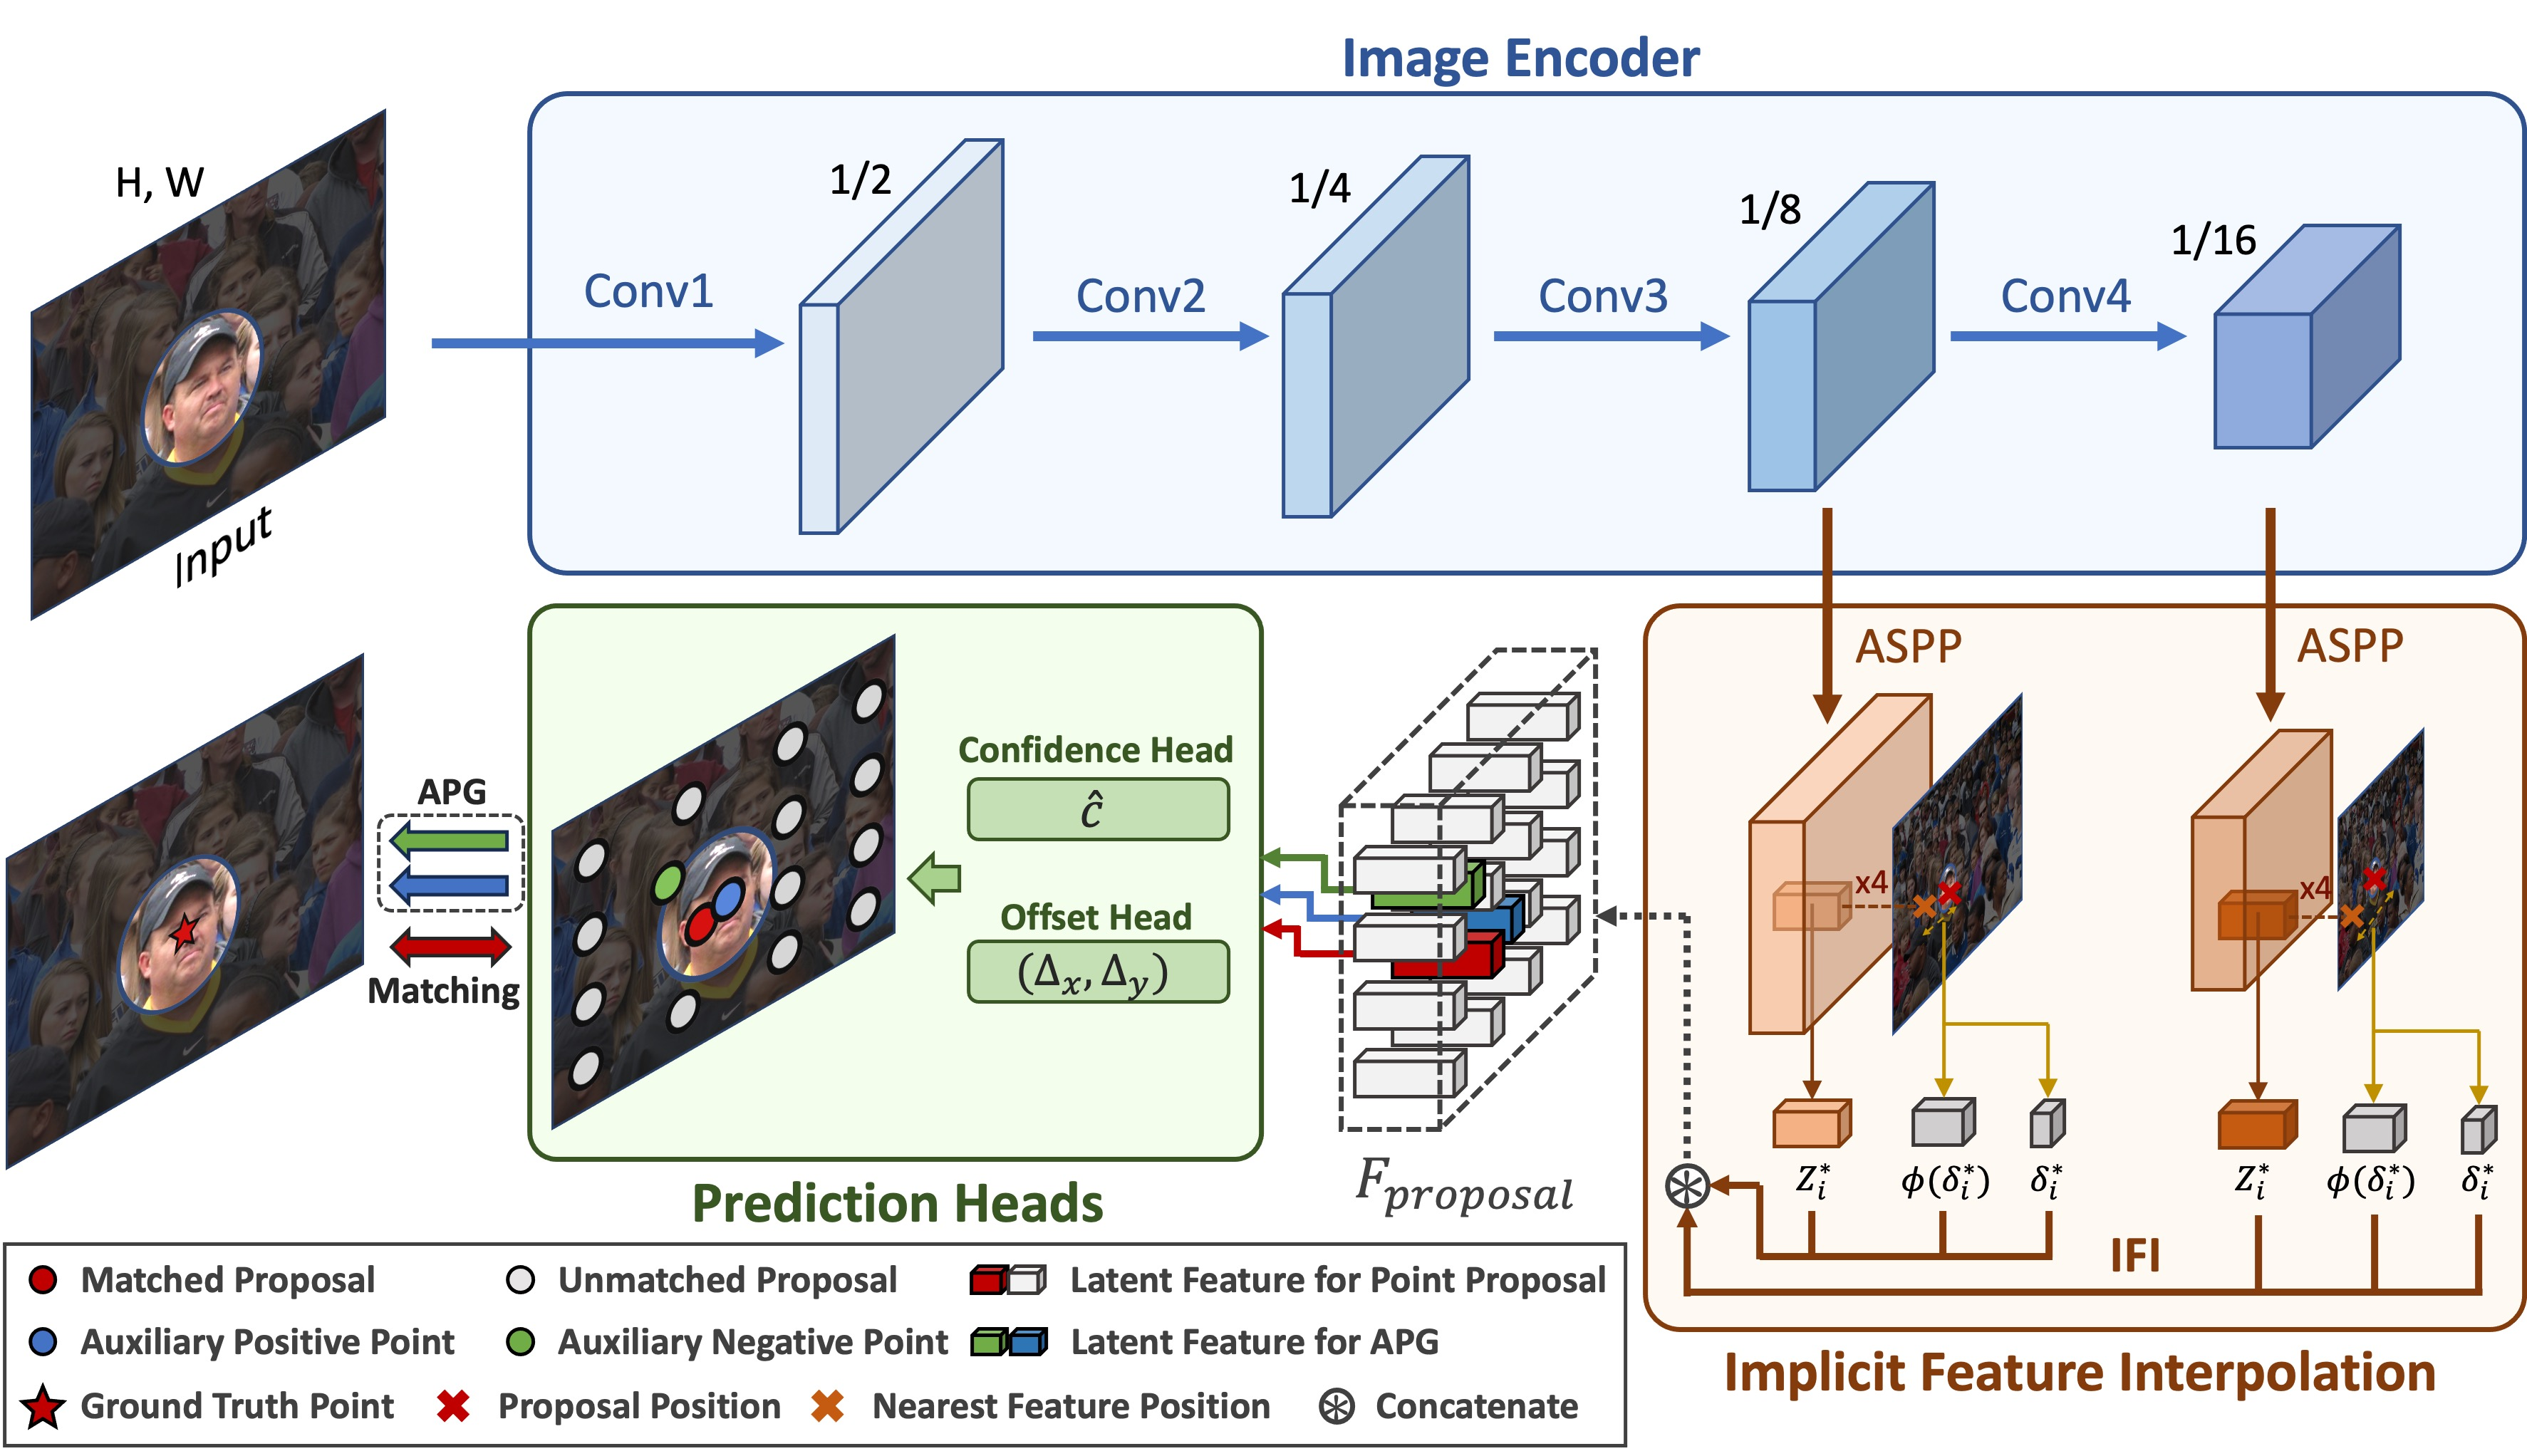
\includegraphics[width=\linewidth]{figures/apgcc_arch}
    \caption{APGCC 整体架构（引自原论文）。图像编码器提取 $1/2$--$1/16$ 多尺度特征，
    IFI（Implicit Feature Interpolation）在连续坐标上隐式插值特征，预测头为每个锚点输出
    置信度 $\hat{c}$ 与坐标偏移 $(\Delta_x,\Delta_y)$，再经匈牙利匹配与真值点一对一关联。
    本次 baseline 采用其编码器、IFI 与预测头主干；图中辅助点引导（APG）分支在 baseline
    中未启用（\texttt{AUX\_EN=False}）。}
    \label{fig:apgcc-arch}
\end{figure}

\begin{figure}[H]
    \centering
    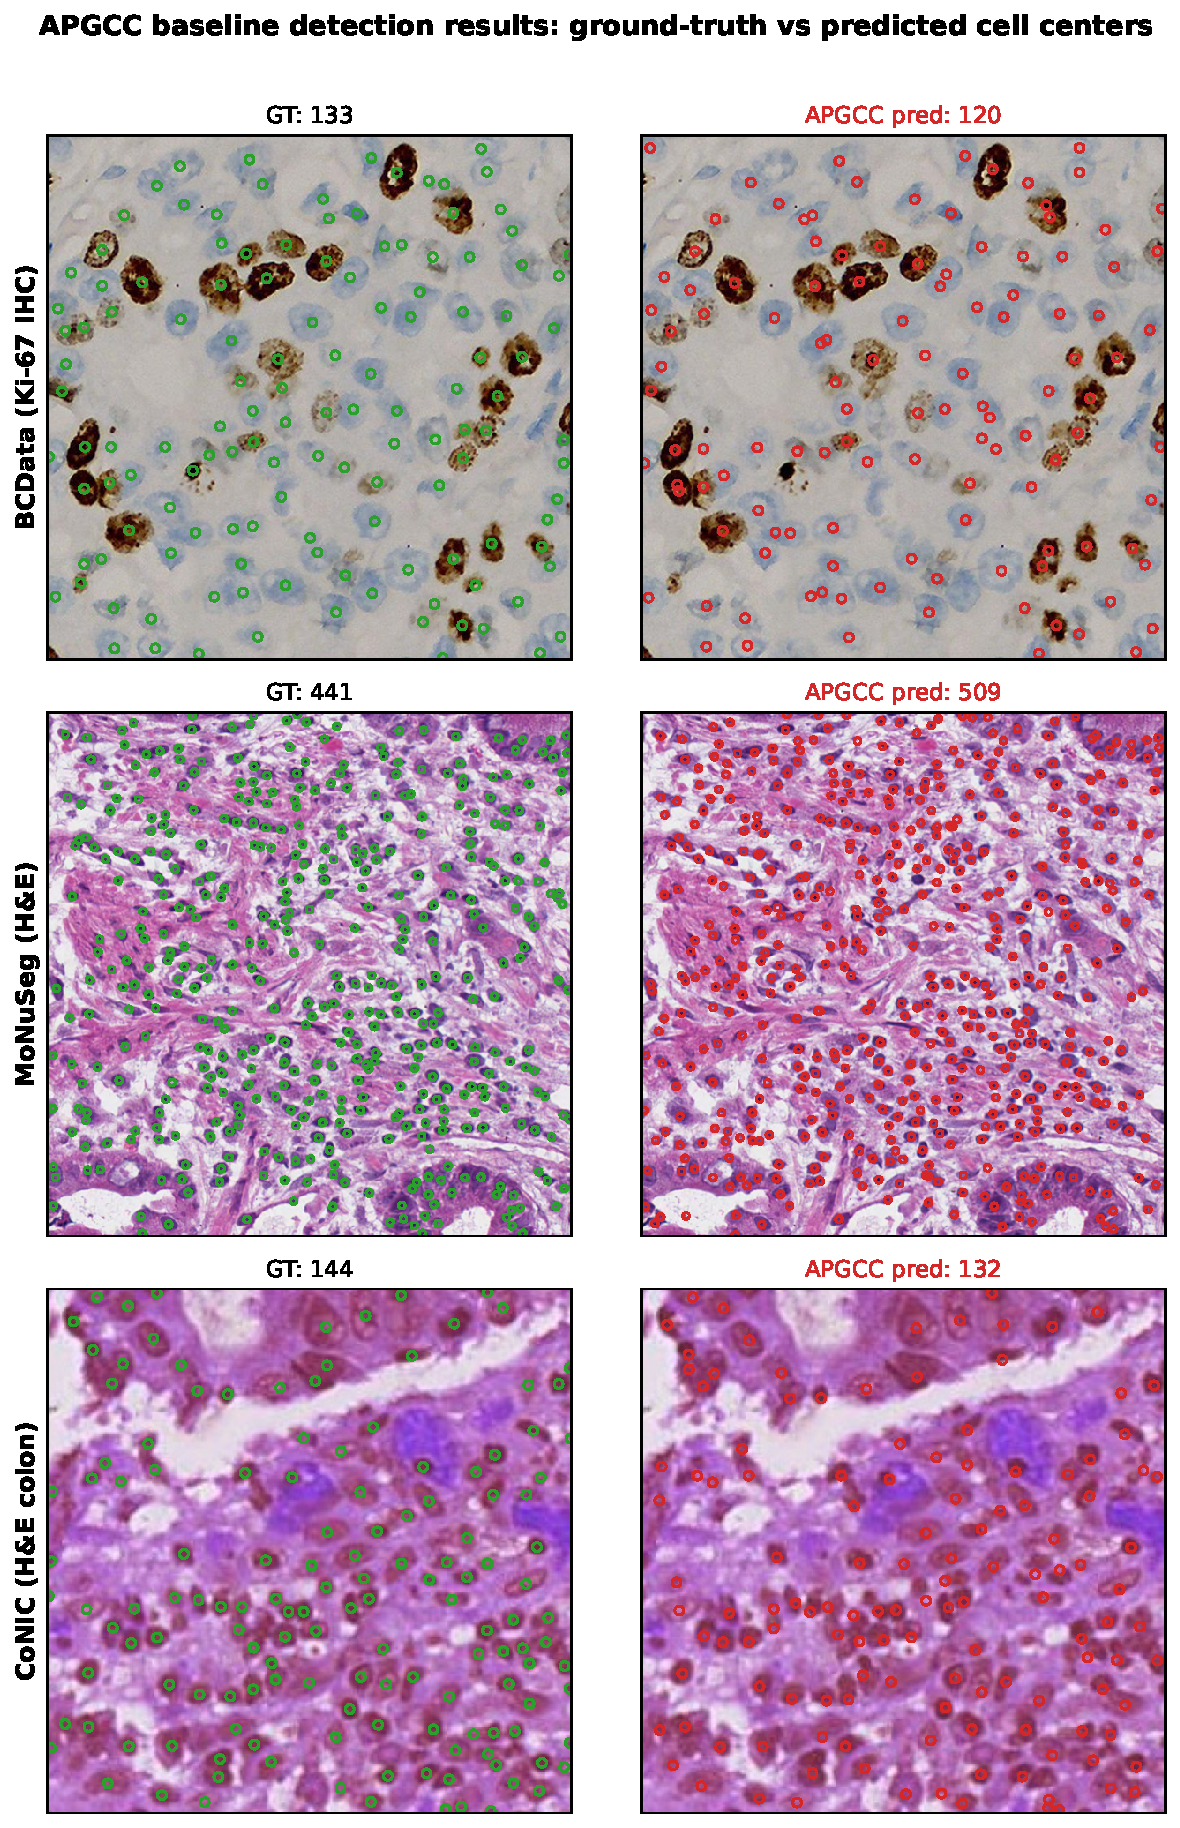
\includegraphics[width=0.74\linewidth]{figures/fig_baseline_detection}
    \caption{APGCC baseline 在三个数据集测试集上的检测结果（代表性整图）。每行一个数据集，
    左列为真值中心点（绿）、右列为 APGCC 预测中心点（红），标题给出对应计数。
    BCData（GT\,$133$/预测\,$120$）、MoNuSeg（GT\,$441$/预测\,$509$）、CoNIC（GT\,$144$/预测\,$132$）
    的预测中心点均与细胞分布吻合，表明点监督框架可直接迁移到病理细胞中心定位与计数。}
    \label{fig:apgcc-detection}
\end{figure}

\begin{figure}[H]
    \centering
    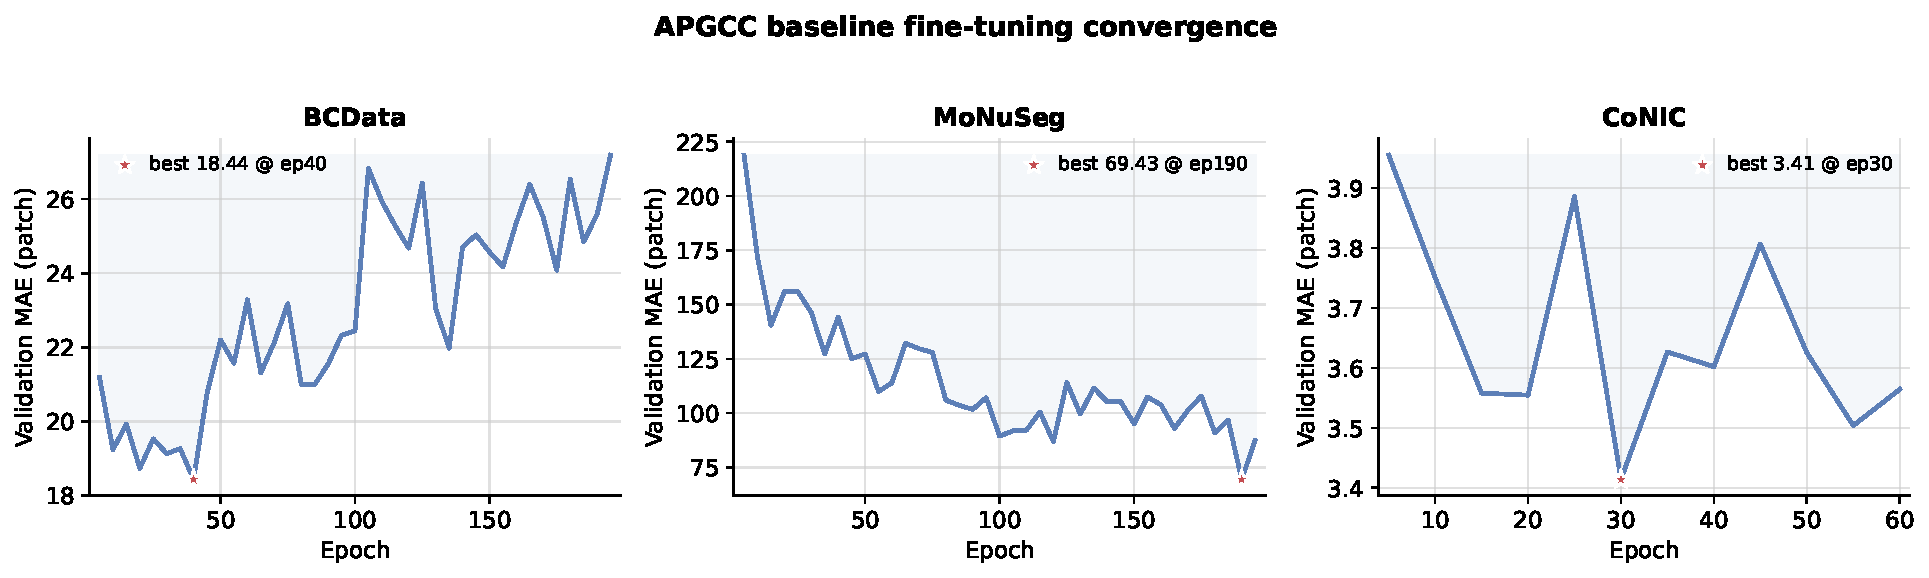
\includegraphics[width=\linewidth]{figures/fig_train_curves}
    \caption{三数据集 baseline 微调的验证 MAE 收敛曲线（红点为最佳轮）。BCData 早收敛后过拟合，
    MoNuSeg 慢且波动，CoNIC 快速收敛——反映尺度/裁剪差异对训练稳定性的影响。}
    \label{fig:apgcc-curve}
\end{figure}

\begin{figure}[H]
    \centering
    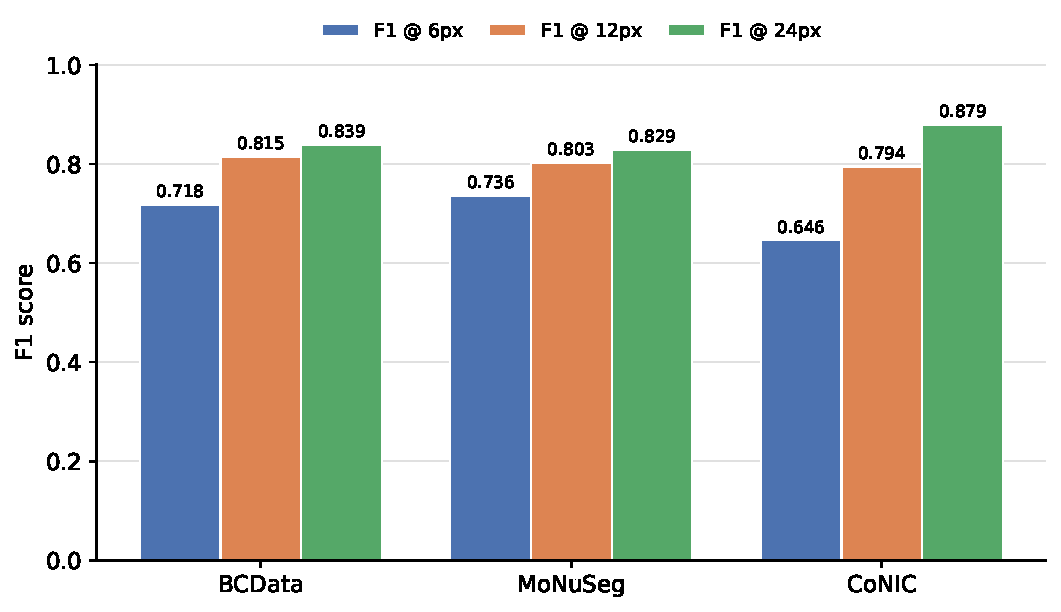
\includegraphics[width=0.74\linewidth]{figures/fig_localization_f1}
    \caption{三数据集 baseline 定位 F1@6/12/24\,px 对比。随匹配半径放宽 F1 提升；
    CoNIC 在 $6$\,px 下最低，体现密集小目标精确定位之难。}
    \label{fig:apgcc-f1}
\end{figure}

\begin{figure}[H]
    \centering
    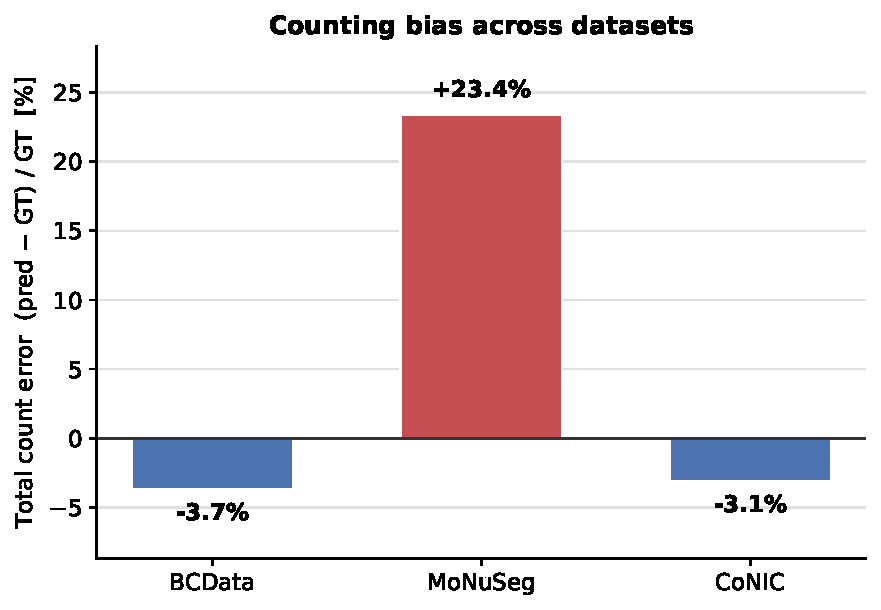
\includegraphics[width=0.62\linewidth]{figures/fig_counting_bias}
    \caption{三数据集 baseline 计数偏差（预测总数相对真值）。MoNuSeg 高密度粘连导致显著过计数，
    BCData/CoNIC 轻微欠计数，说明固定阈值难以适配不同密度分布。}
    \label{fig:apgcc-bias}
\end{figure}

\begin{figure}[H]
    \centering
    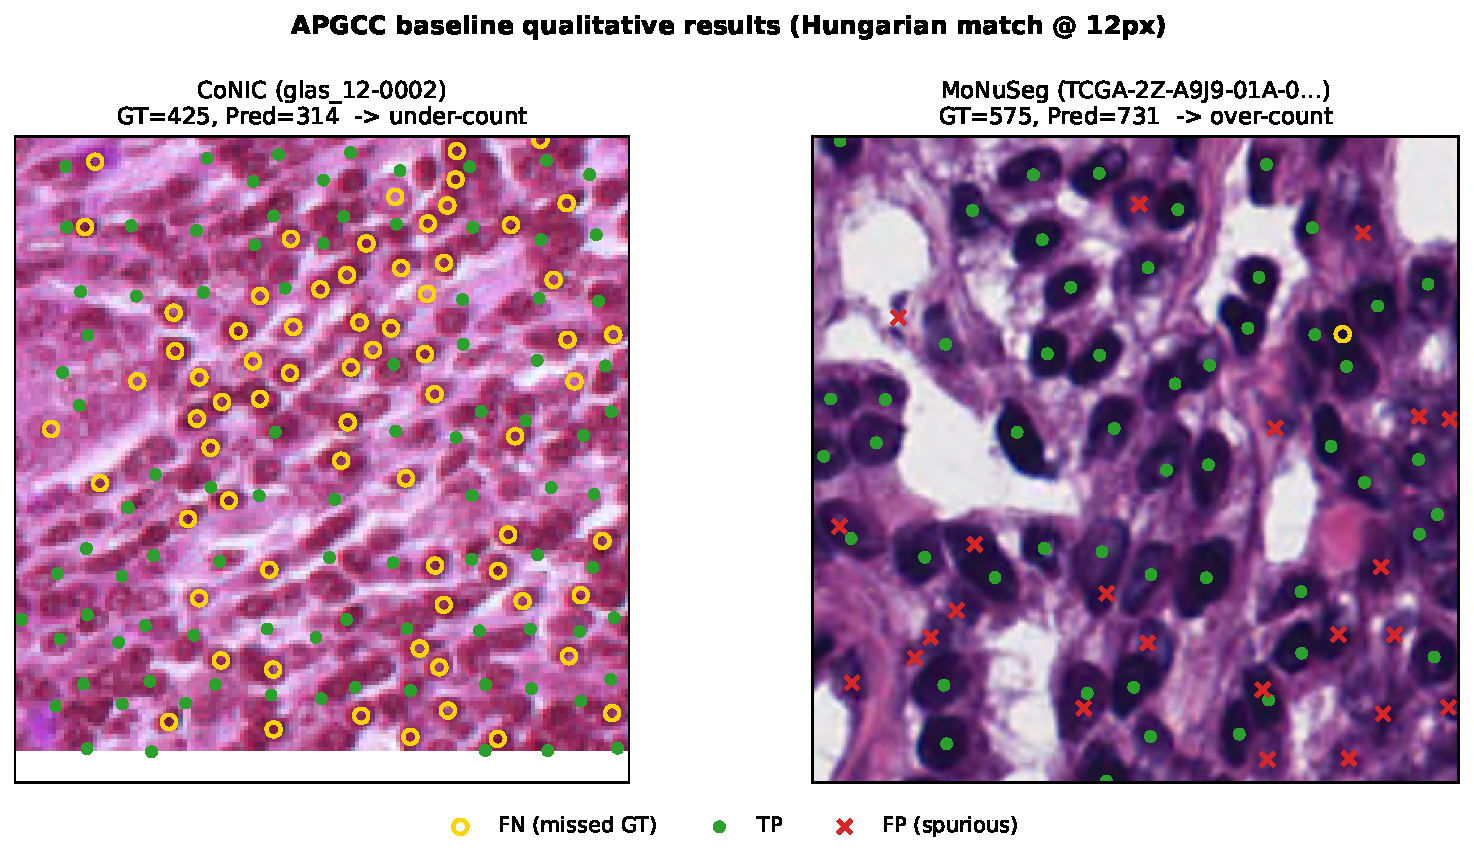
\includegraphics[width=\linewidth]{figures/fig_qualitative}
    \caption{APGCC baseline 定性结果（匈牙利匹配 @ $12$\,px；绿点为 TP、红叉为 FP、黄圈为漏检的 GT）。
    左：CoNIC 密集 patch（\texttt{glas\_12-0002}，GT $425$ / 预测 $314$），密集小目标存在大量漏检，
    对应\emph{欠计数}；右：MoNuSeg 细胞核粘连区（GT $575$ / 预测 $731$），相邻核被重复响应而产生假阳性，
    对应\emph{过计数}。二者直观印证了密度相关的计数偏差。}
    \label{fig:apgcc-qual}
\end{figure}
